\documentclass[a4paper,10pt,twoside]{book}

\usepackage{geometry}
\geometry{top=3cm,bottom=4cm}

\usepackage{ucs}
\usepackage[utf8x]{inputenc}
\usepackage[francais]{babel}
\usepackage[T1]{fontenc}
\usepackage{tabulary}

\usepackage[pdftex]{graphicx}
\usepackage[pdftex]{hyperref}
\hypersetup{%
   a4paper,
   bookmarksnumbered,
   bookmarksopen=true,
   bookmarksopenlevel=0,
   plainpages=false,
   unicode=true,
   colorlinks=true, 
   linkcolor=blue,
   urlcolor=blue,
   pdftitle={Manuel de l'utilisateur},
   pdfsubject={Manuel d'utilisation du logiciel XINX, editeur de feuille de style},
   pdfauthor={Ulrich Van Den Hekke}
}
\usepackage{nameref}
\usepackage{graphicx}
\usepackage{fancybox}
\usepackage{fancyvrb}
\usepackage{alltt}
\usepackage{color}

\author{Ulrich Van Den Hekke}
\date{05/05/2011}
\title{Manuel de l'utilisateur}

\begin{document}
  
\maketitle

\tableofcontents \addcontentsline{toc}{chapter}{Table des matières}

\chapter{Introduction}

XINX est un logiciel de développement essentielement tournée vers l'édition de feuille de style XSL, utilisé pour générer des fichiers HTML. 
Une feuille de style XSL est un fichier qui décrit une liste de transformation à appliquer à chaque noeud d'un fichier XML pour le transformer en un autre fichier text (Text plat, HTML, ou un autre fichier XML). Le domaine de XINX s'est un peu étendue dans l'édition des JavaScript et des feuilles de styles CSS associé à la page XSL.

Bref XINX est fait pour vous aider à développer votre site internet à base de feuille de style XSL.

\begin{center}
 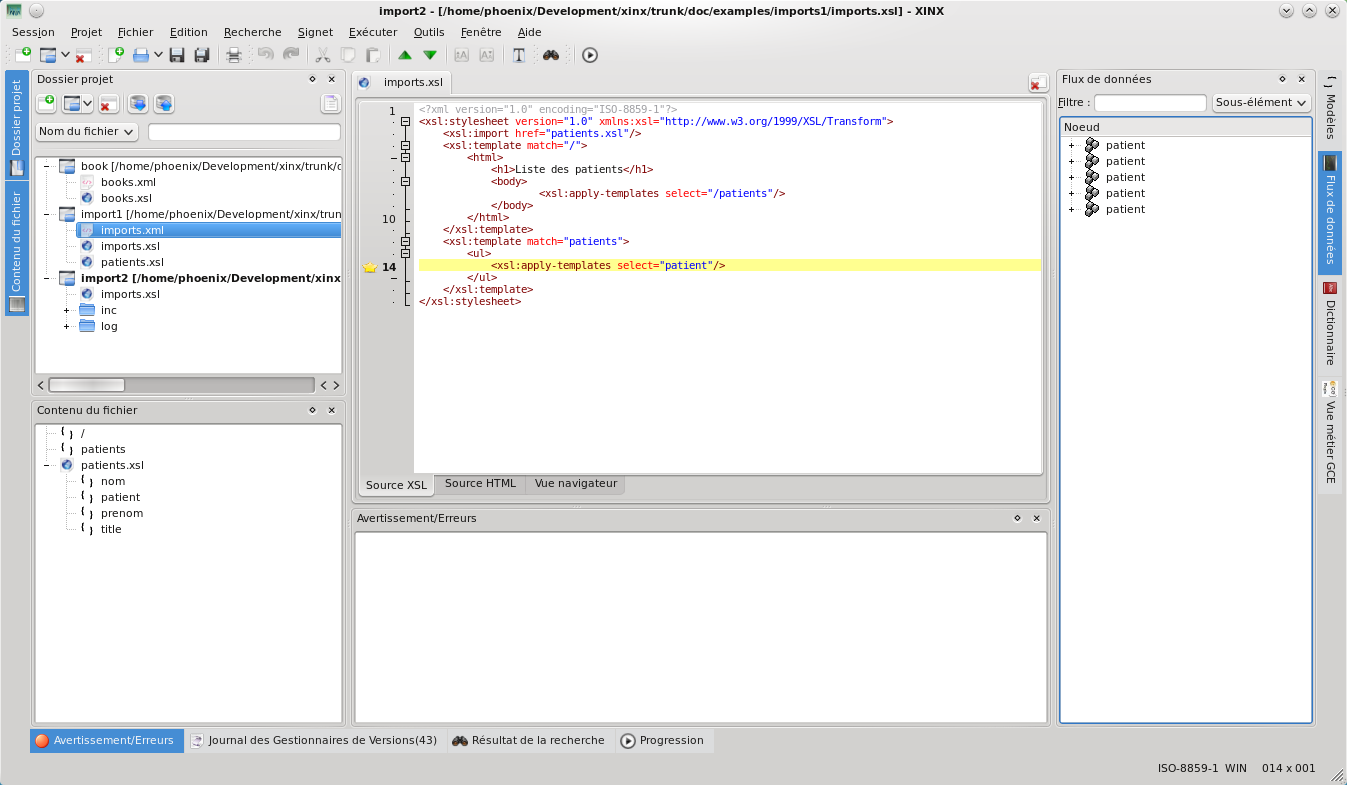
\includegraphics[width=\textwidth]{./mainform.png}
\end{center}

Le logiciel a été écris au début pour le développement des feuilles de styles de la société \href{http://www.generixgroup.com/}{Generix Group} et été fortement tournée vers cette technologie. Maintenant XINX se concentre sur le développement de feuille de style, et tout spécificité lié à la société Generix Group a été déporté dans un plugins.

Le logiciel XINX peut voir ses fonctionnalité étendue à l'aide de modèle (parfois aussi appelé snipet ou template), à l'aide de script (au format ECMAScript, proche de qu'est la JavaScript), ou à l'aide de plugins (écrit en C++ et en utilisant le framework Qt).

XINX utilise le framework \href{http://qt.nokia.com}{Qt} comme base. Ce même framework est utilisé pour développé l'environnement de bureau \href{htpp://ww.kde.org}{KDE}, mais aussi des logiciels connues comme Skype, \ldots. Qt est n'est pas seulement un framework graphique mais propose quelques extentions au langauge C++ à l'aide des signaux, des slots, des pointeurs partagées, des listes, des boucles foreach, \ldots.

Ce manuel à pour but de vous aider à utiliser le logiciel XINX au mieux. Il vous expliquera comment installer le logiciel sur votre ordinateur, comment le paramètrer, puis comme l'utiliser pour développer vos feuilles de style.

\section{Utilisation des feuilles de style}

\section{Terminologie}

\section{Les fonctionnalités}

\chapter{Installation de XINX}

XINX possède différents paquets pour installer suivant l'environnement. Si vous avez déjà installé un logiciel auparavent sur votre système d'exploitation, l'installation vous sera facile. Comme l'installation du logiciel peut varier suivant la platforme, les instructions seront séparés dans plusieurs chapitre.

\section{MS/Windows}

Vous pouvez obtenir la version binaire de XINX pour les systèmes d'exploitations Ms/Windows sur la page de téléchargement du site de XINX à l'adresse \url{http://xinx.shadoware.org/wiki/Download}. 

Le démarrage de l'installation se fait par un double-clique sur le fichier executable de l'installation (nommé \verb+xinx-0.10.1.2531.exe+). Le programme install une version 32-bit de XINX. Il n'existe pas de version 64-bit de XINX.

Le programme vous demandera alors, après l'écran d'accueil, les composants que vous souhaiter installer avec XINX. Voici la liste des composants disponible :

\paragraph{Application et Bibliothèques necessaires} Ce paquet ne peux être déselectionner, il contient l'application et l'ensemble des bibliothèques necessaires à son fonctionnement.
\paragraph{Source de l'application} Ce paquet contient les sources de l'application que vous pouvez utiliser pour consultation, ou pour contribuer. Ce sont les sources qui ont été utilisé pour créer la version que vous installez. Les sources peuvent également être retrouvé sur le referenciel SubVersion. Vous n'êtez pas obligé d'installer ce paquet si vous n'avez pas l'intention de regarder les sources de l'application.
\paragraph{APIs de XINX} Ce paquet contient la documentation technique des différentes classes de XINX. Vous pouvez installer ce paquet si vous souhaiter apporter des modifications à XINX ou développer vos propre plugins.
\paragraph{Mode de fonctionnement Generix} Ce paquet permet d'installer le plugin qui vous permettra d'ajouter les fonctionnalités qui vous seront utils si vous développez des feuilles de style pour l'applicatif GCE. Pour plus d'information vous pouvez vous rendre à la section \ref{sec:Generix}.
\paragraph{Encapsulation de CVS} Ce plugin vous permet de coupler votre projet XINX avec le référenciel CVS. Pour plus d'information vous pouvez rendre à la section \ref{sec:RCS}. Il est necessaire d'avoir installer CVSNT pour pouvoir utiliser ce plugin.
\paragraph{Encapsulation de SubVersion} Ce plugin vous permet de coupler votre projet XINX avec le référenciel SubVersion. Pour plus d'information vous pouvez vous rendre à la section \ref{sec:RCS}. Il est necessaire d'avoir un client SubVersion d'installer (commande \verb+svn.exe+).
\paragraph{Plugin SubVersion pour XINX} Ce plugin vous permet de coupler votre projet XINX avec un référenciel SubVersion. Pour plus d'information vous pouvez vous rendre à la section \ref{sec:RCS}. Ce plugin ne necessite aucune dépendance. Vous pouvez alors utiliser SubVersion directement.
\paragraph{Appel de WebServices de type RPC} Ce plugin vous permet d'appeler des Services Internet de type RPC directement depuis XINX. Pour plus d'information vous pouvez vous rendre à la section \ref{sec:Services}.
\paragraph{Quelques scriptes} Ce paquet contient quelques scriptes utilitaire pouvant être appelé depuis XINX. Ces scripts sont écris dans un language proche du JavaScript. Voir la section \ref{sec:Scripts}.

Le programme d'installation créera un group XINX dans le menu <<Démaré>> de Windows qui vous permettra de lancer l'application et d'accéder à la documentation. Il vous sera également possible d'associer les fichier d'extentions \verb+.xsl+, \verb+.js+, et \verb+.fws+ avec XINX pour ouvrir automatiquement ce dernier lors du double clique sur un fichier portant l'une de ces extentions.

\section{Gnu/Linux}

\subsection{Version binaire pour Gnu/Debian}

Une version binaire de XINX est disponible pour la distribution Gnu/Debian. Vous pouvez la télécharger en ajoutant le dépôt \verb+http://apt.shadoware.org/+ à votre fichier \verb+/etc/apt/sources.list+ puis executant la commande d'installation de XINX. Votre gestionnaire de paquet s'occupera alors d'installer automatiquement les paquets manquants. 

XINX pour fonctionner necessite Qt, et les librairies libxml2 et libxslt1 de gestion des fichiers XML.

\begin{verbatim}
# echo "deb http://apt.shadoware.org/ squeeze main" >> /etc/apt/sources.list
# aptitude install xinx
\end{verbatim}

Vous pouvez alors démarrer XINX depuis le menu ou en le lancement depuis la ligne de commande. 

\subsection{Version source pour les autres distribution}

\paragraph{Récupérer les sources :}

Pour les autres distribution Gnu/Linux, il n'y a pas de paquet de disponible actuellement, il est néanmoins très facile de compiler XINX à partir des sources. Vous pouvez récupérer les sources de XINX sur la page de téléchargement à l'adresse \url{http://xinx.shadoware.org/wiki/Download}. Le fichier se présentera sous forme d'une archive \verb+.7z+. Vouz pourrez décompresser l'archive à l'aide de la commande :

\begin{verbatim}
# mkdir xinx
# cd xinx
# 7z x ../xinx-0.10.1.2531.7z
\end{verbatim}

\paragraph{Compilation :}

Sous Gnu/Linux la compilation necessite l'installation des paquets suivants\footnote{les paquets sont à titre d'exemple, il faudra adapter la liste des paquets enfonction de votre distribution.} :
\begin{itemize}
 \item libxml2-dev
 \item libxslt1-dev
 \item cmake
 \item libqt4-dev
 \item libsvncpp-dev 
\end{itemize}

Placer vous ensuite dans le dossier parent au dossier xinx et lancer la compilation à l'aide des commandes suivante :
\begin{verbatim}
# mkdir xinx-build
# cd xinx-build
# cmake ../xinx
# make
# sudo make install
\end{verbatim}

Si tout les paquets sont disponible la compilation et l'installation se passeront sans problème. En cas d'erreur, corrigé les paquets manquant et recommncer depuis le début.

\chapter{Interface principale de XINX}

Après l'installation, vous pouvez démarrer XINX comme suite :
\begin{itemize}
 \item Sous Windows, dans le menu << Démarrer >>, cliquez sur le programme dans le groupe XINX. Sous Vista et supérieur, vous pouvez aussi écrire directement <<XINX>> dans la boite de recherche du menu << Démarer >>
 \item Sous Linux, selon votre bureau, vous retrouver le programme XINX dans le groupe <<Developpement>> de votre menu d'application. Vous pouvez également tapper XINX dans le lanceur rapide ou dans une console Linux. 
\end{itemize}

Quand vous démarrez XINX pour la première fois, une fenêtre de configuration devrait s'ouvrir :

\begin{center}
 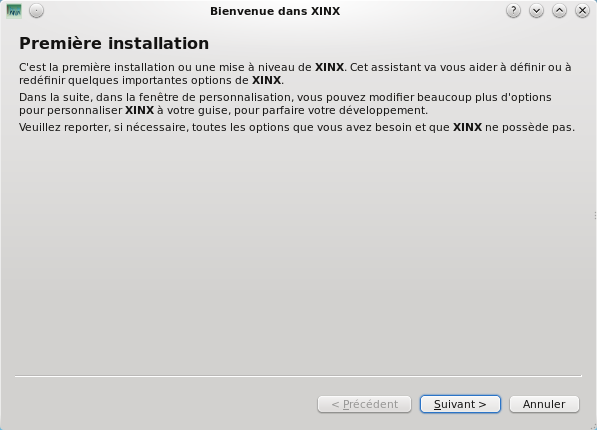
\includegraphics[width=0.60\textwidth]{./firstinstall1.png}
\end{center}

Cette fenêtre vous permettra de configurer les principales fonctionnalités de XINX. 

\begin{center}
 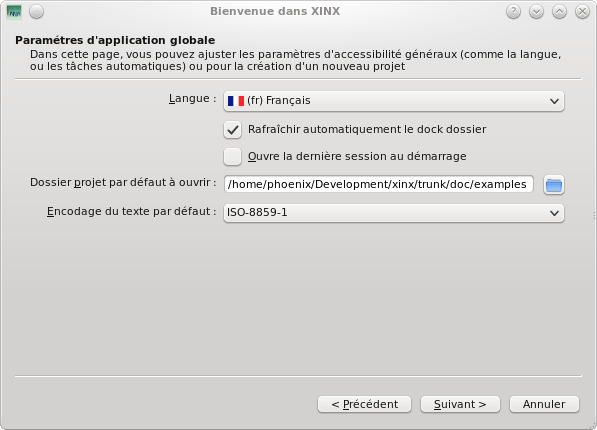
\includegraphics[width=0.60\textwidth]{./firstinstall2.png}
\end{center}

\paragraph{Langue} Sur la première page vous allez pouvoir choisir la langue d'affichage de XINX. 

\paragraph{Rafraichir automatiquement le dock dossier} Si vous décochez cette case, lorsque vous rechercherez un fichier dans un projet, il vous faudra frapper la touche <<Entrer>> pour lancer la recherche, sinon elle se lancera automatiquement à la fin de la frappe.

\paragraph{Ouvrir la dernière session au démarrage} Vous pouvez également indiquer que XINX doit ouvrir la dernière session au démarrage, avec les derniers projets ouvert. Si vous ne souhaiter pas ouvrir la dernière session au démarrage, XINX vous proposera dans une boîte de dialogue la liste des sessions disponible ainsi que la liste des projets possible.

\paragraph{Dossier projet à ouvrir par défaut} Le <<Dossier projet à ouvrir par défaut>> est le dossier qui vous sera proposé lorsque que vous allez créer un nouveau projet. C'est généralement le dossier qui se trouve au dessus de tous les dossiers sur lesquels vous allez travailler.

\paragraph{Encodage du texte par défaut} est l'encodage par défaut à utiliser pour les fichier dont XINX ne peux déterminer l'encodage (fichier texte, fichier JavaScript, \dots). Cette option n'a aucune effet sur les fichiers XML définissant au début du fichier l'encodage à utiliser.

\begin{center}
 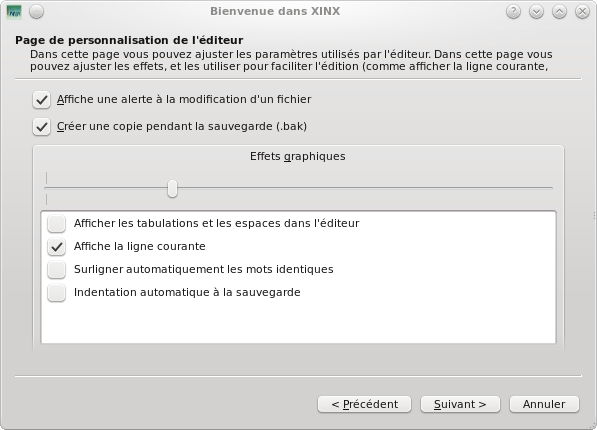
\includegraphics[width=0.60\textwidth]{./firstinstall3.png}
\end{center}

Sur l'écran suivant vous allez trouver différentes options lié à l'édition du texte. Si vous êtes familier avec d'autres IDE, vous reconnaitrez des options. 

\paragraph{Afficher une alerte à la modification d'un fichier} Lorsqu'un programme externe modifie un fichier ouvert dans XINX, ce dernier vous demandera alors automatiquement de recharger le fichier. 

\paragraph{Créer une copie pendant la sauvegarde (.bak)}

\paragraph{Afficher les tabulations et les espaces dans l'éditeur}

\paragraph{Surligner automatiquement les mots identiques}

\paragraph{Indentation automatique à la sauvegarde}

\begin{center}
 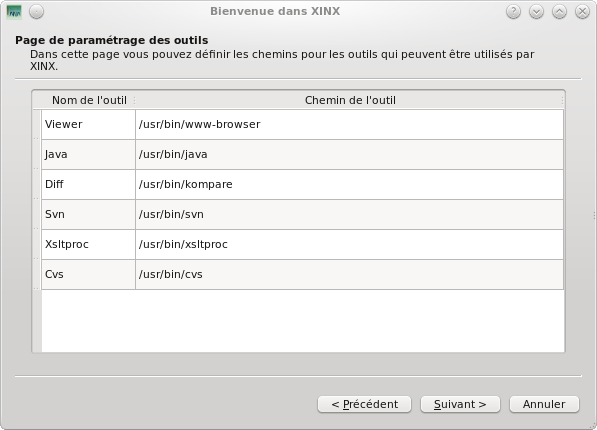
\includegraphics[width=0.60\textwidth]{./firstinstall4.png}
\end{center}

\section{Configuration de XINX}

\section{Les projets}

\subsection{Création d'un projet}

\subsection{Utilisation des projets}
\label{sec:RCS}
Gestionnaire de version


\section{Mode édition}

\subsection{Edition}

\subsection{Test}

Flux de donnée / présentation

\section{Les onglets}

\chapter{Les modèles}

\chapter{Les scriptes}
\label{sec:Scripts}

\chapter{Les extentions}

\section{Services}
\label{sec:Services}

\section{Generix}
\label{sec:Generix}

\appendix
\chapter{Les raccourcis}

\chapter{Interface ECMAScript de XINX}

\chapter{Point de vue technique}

\section{Où sont stocker les fichiers de XINX}

\chapter{Dépannage}

\chapter{Limitations connues}

\chapter{Logiciels tiers et licence}

\chapter{Glossaire}

\end{document}
